\begin{enumerate}[label=\thesection.\arabic*.,ref=\thesection.\theenumi]
\numberwithin{equation}{enumi}

\item A second-order real system has the following properties
\begin{enumerate}
\item the damping ratio $\zeta=0.5$ and undamped natural frequency $\omega_n=10$rad/s 

\item  the steady state value of the output, to a unit step input, is 1.02.
\end{enumerate}

Find the transfer function of the system. 
\\
\solution The general transfer function of a second order system is given by \eqref{eq:ee18btech11012_second}
%
\begin{align}
H(s)=\frac{k\omega^2}{s^2+2\zeta\omega+\omega^2}
\end{align}
%
From the given information, 
\begin{align}
\zeta&=0.5
\\
\omega&=10
\\
    c(\infty)&=\lim_{s \to 0}s\frac{kH(s)}{s} = 1.02
\\
\implies     c(\infty)&=k=1.02
\end{align}
%
using the final value theorem, where $c(t)$ is the step response.  
$\therefore$, transfer function of the system is
\begin{align}
H(s) =     \frac{102}{s^2+10s+100}
\end{align}
The step response of the transfer function  is 
\begin{multline}
c(t)=e^{-5t}\lcbrak{\brak{\frac{-51}{50}}\cos(5\sqrt{3}t)}\\
-\rcbrak{\brak{\frac{17\sqrt{3}}{50}}\sin(5\sqrt{3}t)}+\frac{51}{50}u(t)
\end{multline}
The following code plots the step response in Fig. \ref{fig:es17btech11015}.
\begin{lstlisting}
codes/es17btech11015.py
\end{lstlisting}
\begin{figure}
\centering
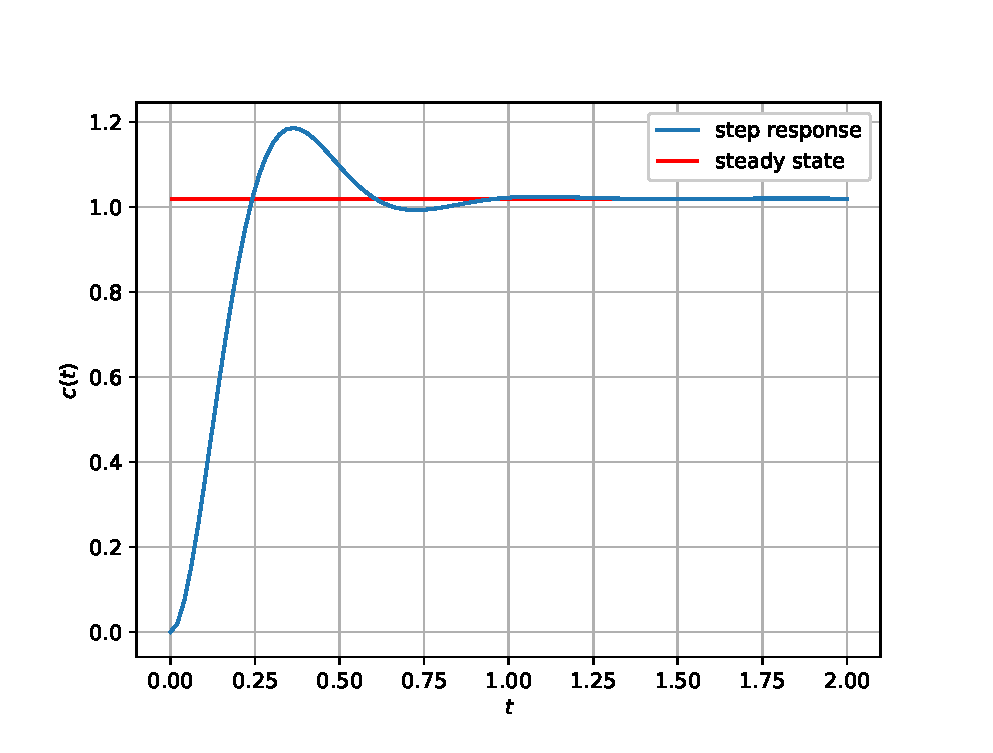
\includegraphics[width=\columnwidth]{./figs/es17btech11015.eps}
\caption{}
\label{fig:es17btech11015}
\end{figure}
\end{enumerate}
